% TODO: Say we can load pgm maps from ROS 2

\section{Simple Simulator}
The simple simulator was developed as an easy way to test and debug the behavior of a robot swarm given a robot behavior. It runs a simple 2D simulation with a time step of 60 steps pr. simulated second in a multi threaded manner. Robots are represented as circles, with their id marked in the middle. 
\Cref{fig:simple-sim-interface} shows the user interface if the simple simulator.

\begin{figure}[H]
    \begin{center}
        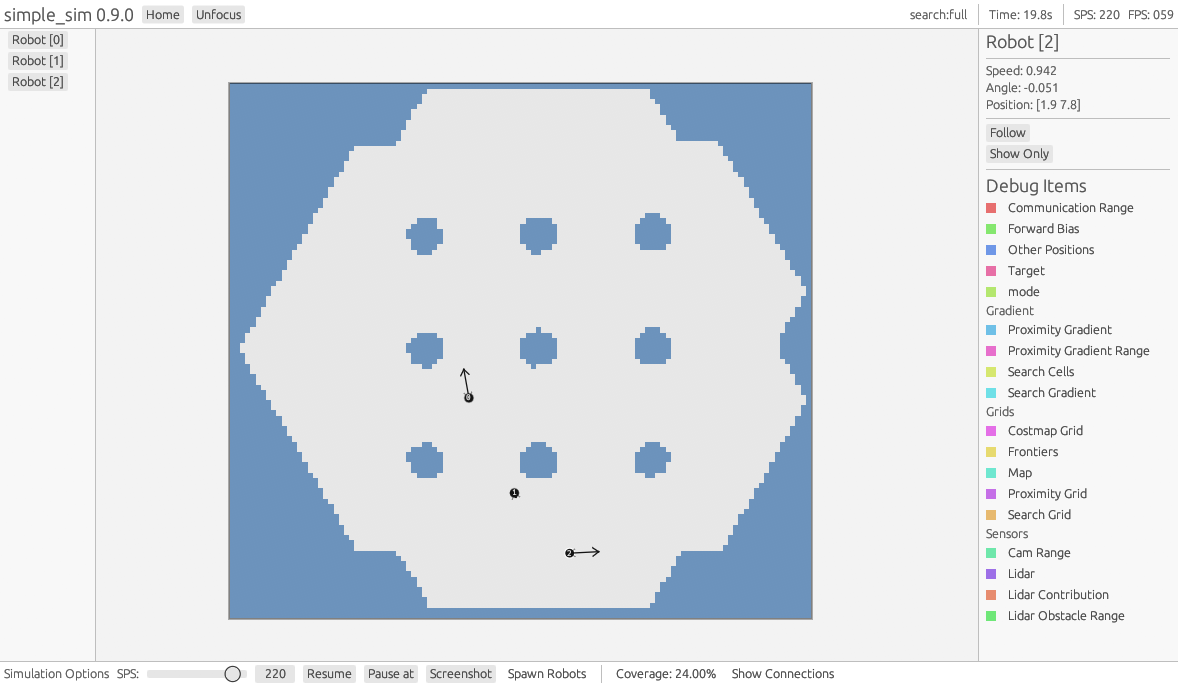
\includegraphics[width=0.95\textwidth]{figures/simple-sim-gui.png}
    \end{center}
    \caption{Simple simulator interface as it simulates three robots in the left part of the map.}\label{fig:simple-sim-interface}
\end{figure}

\subsection{Sensor Approximation}
Running a robot's behavior requires pose, LiDAR, and camera inputs. The pose is set directly by the simulator and therefore does not require significant implementation effort. Both LiDAR and camera sensors are approximated using ray marching techniques {\color{red}[CITE]}. \\

LiDAR is simulated by casting rays radially around the robot at fixed angular intervals. Each ray is marched forward until it intersects with an object, as illustrated in \cref{fig:lidar-approximation}. \\

The camera is approximated similarly to the LiDAR, but with constraints imposed by a defined field of view. The field of view is configured to match that of the Turtlebot 4 camera. Unlike full camera simulation, no object detection algorithm is applied. When a ray intersects an object, the nature of the object, such as whether it is an obstacle or a target, is inferred directly.

\begin{figure}
    \centering

    \begin{subfigure}[b]{0.45\textwidth}
        \centering
        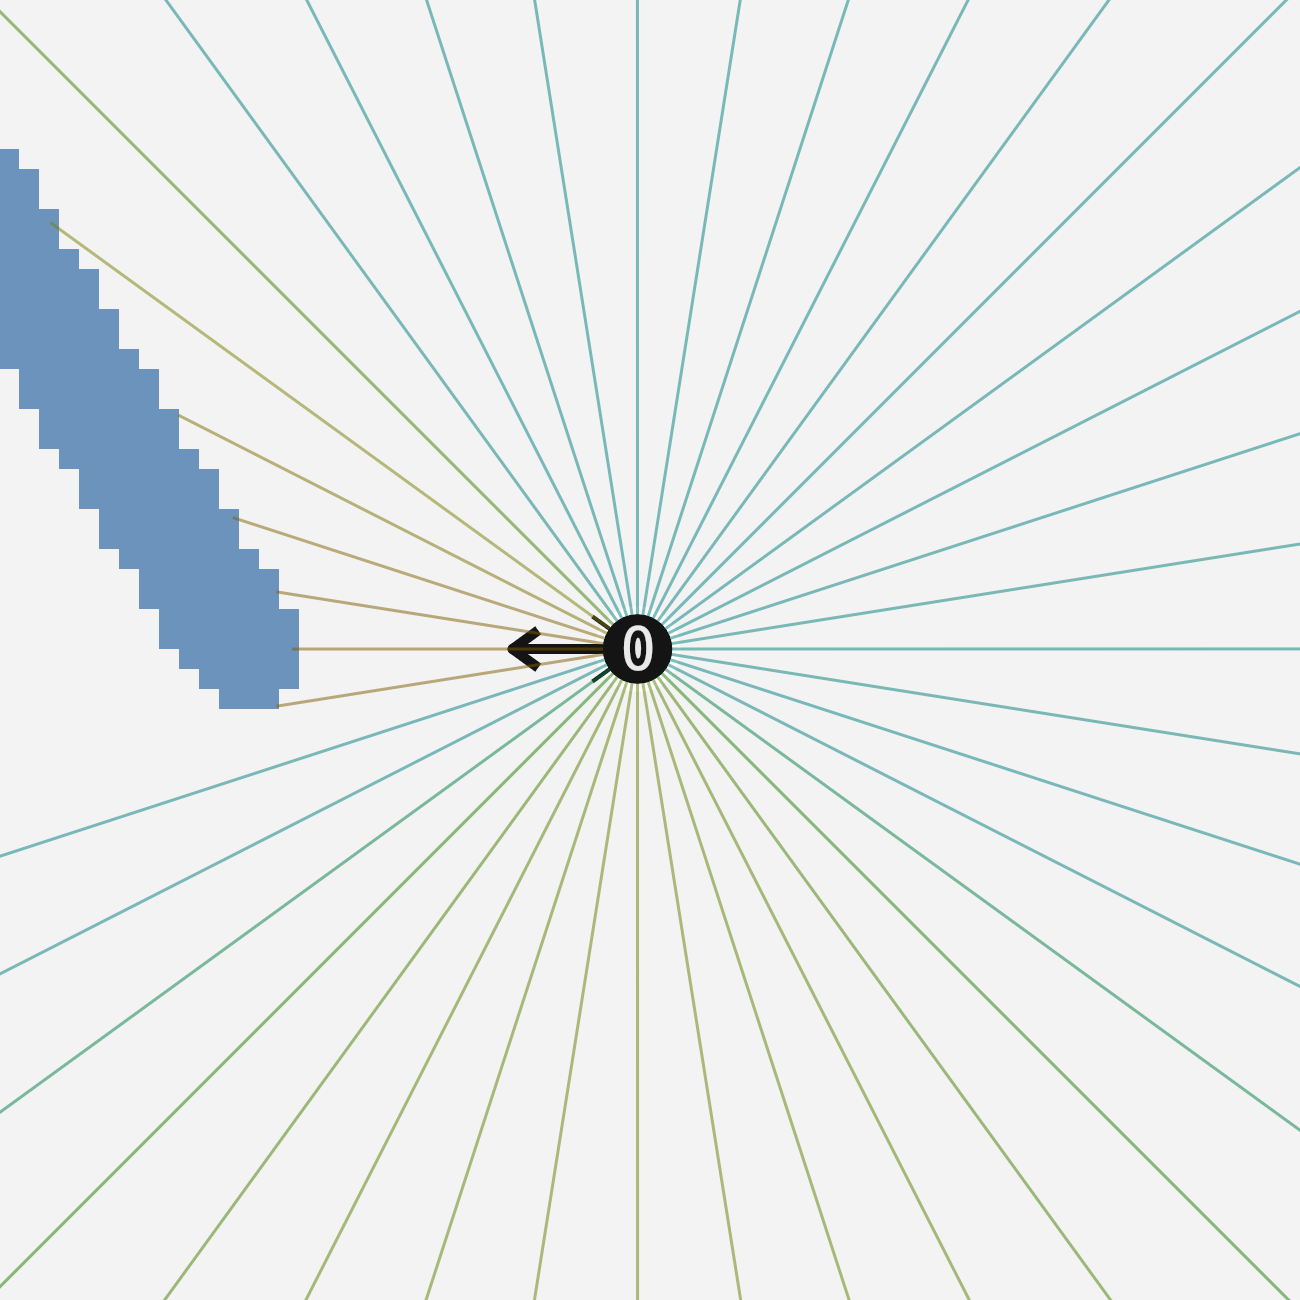
\includegraphics[width=\textwidth]{figures/simple-lidar.png}
        \caption{LiDAR approximation}
        \label{fig:lidar-approximation}
    \end{subfigure}
    \begin{subfigure}[b]{0.45\textwidth}
        \centering
        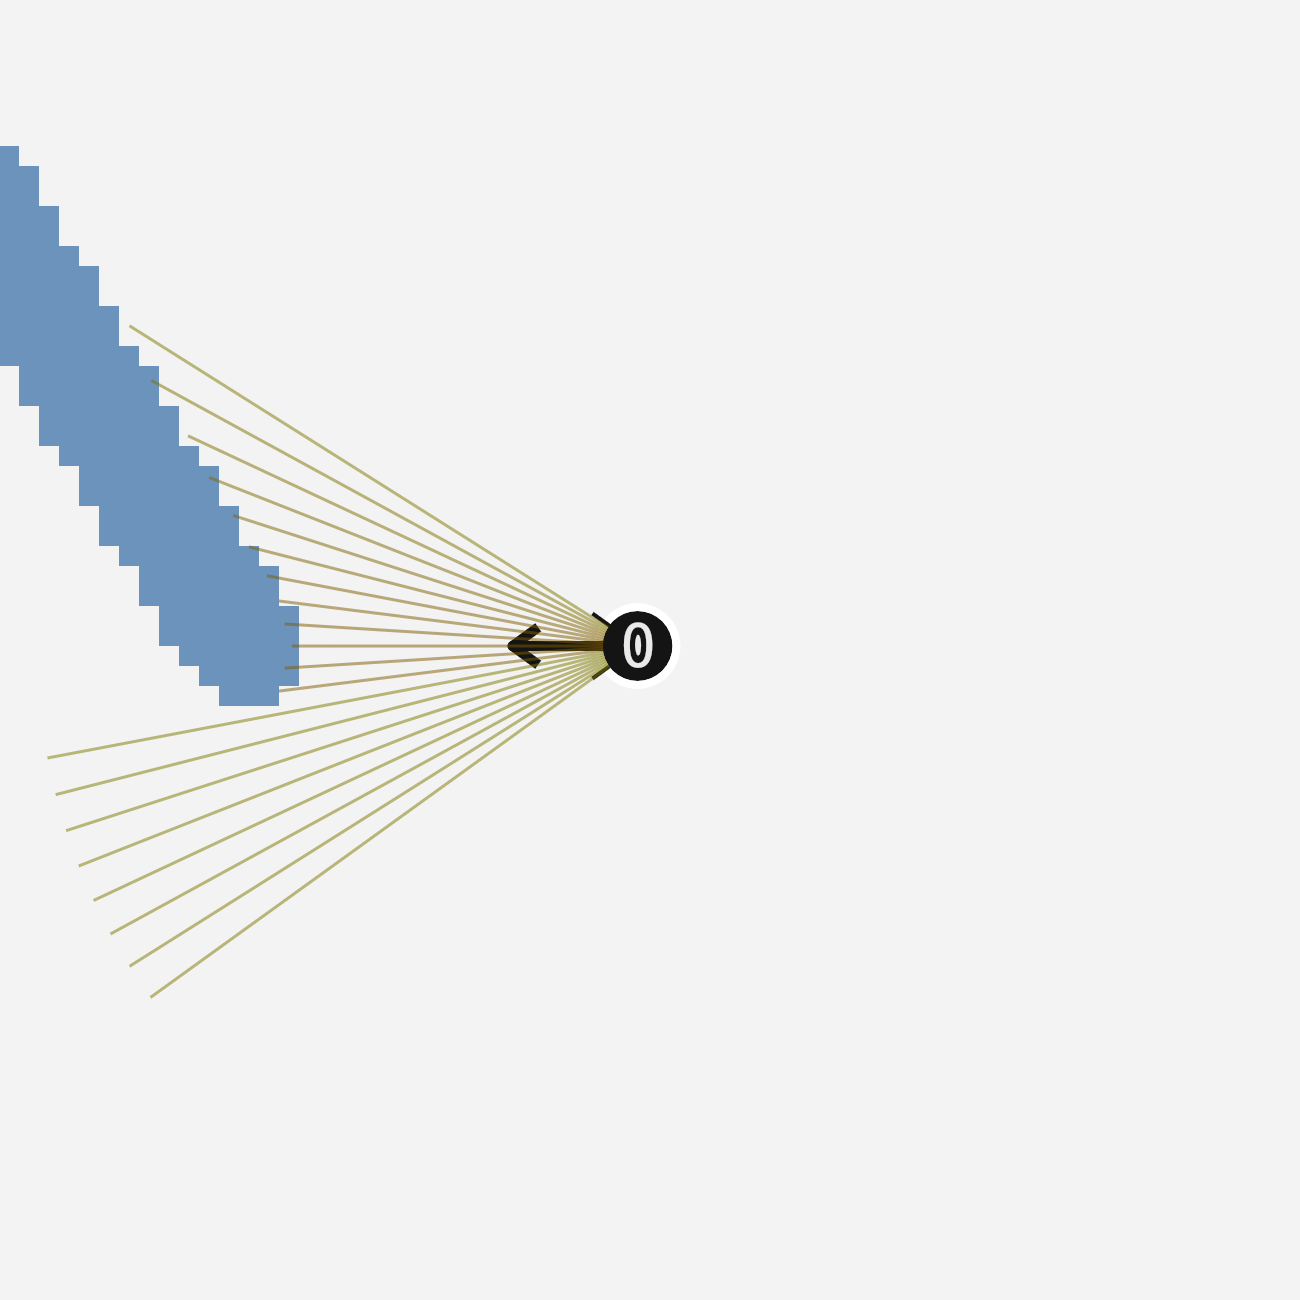
\includegraphics[width=\textwidth]{figures/simple-camera.png}
        \caption{Camera approximation}
        \label{fig:camera-approximation}
    \end{subfigure}

    \caption{LiDAR and camera simulated in the simple simulator.}\label{fig:sensor-approximation}
\end{figure}

\subsection{Debugging}
To obtain debugging information and verify the correctness of the robot's behavior, the simple simulator can be used to inspect both the behavior and the internal state of the robots. \texttt{Botbrain} provides a debugging interface called \texttt{Debug Soup}. This interface is based on the principle that each debug item has a category and a key for access. Various elements such as grids, paths, goals, and more can be added from the robot behavior and visualized in either \texttt{simple\_sim} or ROS 2.

% TODO: Library
